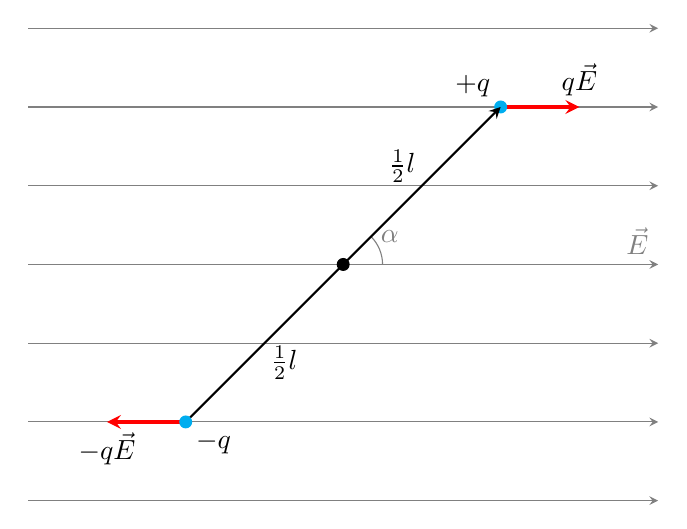
\begin{tikzpicture}[>=stealth]
	\foreach \y in {-3,-2,...,3}
		\draw[-latex, thin, gray, ->] (-4, \y) -- (4, \y);
	\node[gray, above left] at (4, 0) {$\vec{E}$};

	\draw[fill] (0, 0) circle [radius=0.075];

	\node at (0.75, 1.25) {$\frac{1}{2}l$};
	\node at (-0.75, -1.25) {$\frac{1}{2}l$};

	\draw[gray] (0.5, 0) arc [radius=0.5, start angle=0, end angle=45] node[right] {$\alpha$};

	\draw[red, very thick, ->] (-2, -2) -- (-3, -2) node[black, below] {$-q\vec{E}$};
	\draw[red, very thick, ->] (2, 2) -- (3, 2) node[black, above] {$q\vec{E}$};
	\draw[cyan, fill] (2, 2) circle [radius=0.075];
	\draw[thick, ->] (-2, -2) node[below right] {$-q$} -- (2, 2) node[above left] {$+q$};
	\draw[cyan, fill] (-2, -2) circle [radius=0.075];

\end{tikzpicture}
